\chapter{Theoretical Framework} % Main chapter title

\label{Chapter:ConceptualFramework}

This section of the report provides with an overview of urban agriculture and its objectives with a theoretical framework of a sustainable city.

\section{Overview of urban agriculture}

The Food and Agricultural Organization defines urban agriculture as any production in the home or within urban area \cite{FAO2003}. In relation to the FAO definition of urban agriculture is the understanding that urban agriculture also implements the practices of farming and gardening in rural areas \cite{Opitz2016}. Some organisations limit their description of urban agriculture to gardens and farms within the inner city \cite{NewYorkN.Y..DepartmentofParksandRecreation.2010}, others include agricultural activities in the urban periphery area \cite{Mok2014}. Thebo, Drechsel, and Lambin \cite{Thebo2014} state a distinction between urban agriculture and urban periphery agriculture based on geographical location. Thebo et al. indicate that urban periphery agricultural activities take places within a distance of 10 to 20 $Km$ of the urban boundary. Based on Thebo's et al. distinction, the present paper addresses only agricultural activities that take place within an urban boundary. The work of Ayambire et al. \cite{Ayambire2019} gives a detailed distinction between urban and urban periphery agriculture.

The purpose of urban agriculture varies between cities. In the northern globe, people farm typically for recreational reasons although farming for household food supply \cite{McClintock2010}. In the southern globe, farming is mainly to satisfy household food needs and other commercial reasons \cite{Amponsah2016, McClintock2010}. Normally, households in the cities in the global south farm mainly for household consumption. On the other hand, rooftops, balconies and parks are used for agricultural purposes within the cities in the global north \cite{McClintock2010}. In this context, urban agriculture is implemented in this paper to study crop farming done through community gardens, backyard gardens and rooftops.

\section{Conceptualising a sustainable city}

The concept of sustainable cities originated in the United Nations World Commission on Environment and Development's (UNWCED) idea of sustainable development. The UNWCED summarised sustainable development as meeting the needs of the present generation without compromising the ability of future generations to meet their own needs. The concept has been a standard to address many areas of human activity. Sustainable cities determines the way humans shall interact with nature, as well as the way human shall take responsibility towards one another and future generations \cite{Yigitcanlar2015}. Lew, Ng, and Ni \cite{Lew2016} suggest that numerous definitions of sustainability and sustainable development are vague due to the varied understanding of sustainable development and the numerous definitions of sustainability \cite{Mebratu1998}. "Environmental economists believe in economic reductionism by undervaluing ecological goods while social ecologist is reductionist-holistic by focusing on the domination of people and nature." \cite{Mebratu1998} These lead to the separation of nature, economy and society, which is problematic for sustainability purposes. This report focus on sustainable development considers its tripartite dimension (economic, social and environmental).

The 11th SDG (Sustainable Development Goal) amplifies the sustainable city definition, which is “to make cities and human settlements inclusive, safe, resilient and sustainable. The concept is influenced by the rapid urbanisation of the world and the effects on the environment. The implication is that sustainability should be an imperative objective in every development plan. In this regard, the main goal of urban development shall be to make cities and ecosystems sustainable \cite{Hiremath2013}.

The compact city concept describes a city that is energy-efficient and less polluting due to the proximity of houses to the commercial areas and work places. The focus is on high density cities, which will result in less commute, efficient transportation and decreased emissions \cite{Abdullahi2015}. Typically, compact cities have less space for green-infrastructure due to the space limitations that have a negative effect on the quantity and quality of vegetation. Liu et al. have shown that compactness can have negative effects on domestic spaces, affordable shelter, and increased crime levels \cite{Liu2017}. These effects contradict the principles of a sustainable city, which target a balance among economic development, environmental protection, and equity in income, employment, shelter, services, infrastructure and transportation \cite{Hiremath}. For this reason, Garden Gem is not intended (but not limited) to be used within a compact city environment.

Models and indices are also based on conceptual terms. For that reason, the following lists the strengths and weaknesses of three indicators to measure a sustainable city. The use of indicators allow a detailed and quantitative way to measure sustainability within a city. This report reviews the existing models (the Green City Index, Global City Indicators Facility and the Global Compact Cities Circles of Sustainability) to develop a framework for a sustainable city. The framework intention id to serve as the basis for the role of urban agriculture in sustainable cities.

\subsection{The Green City Index}

The Green City Index is known as one of the robust models for the identification of a sustainable city \cite{Huang2015}. It comprises thirty indicators, grouped in eight categories. The categories comprise

\begin{itemize}
    \item Environmental governance
    \item Carbon dioxide (CO2)
    \item Buildings
    \item Transport
    \item Water
    \item Waste and land use
    \item Energy
    \item Air quality (refer to Appendix \ref{AppendixA}).
\end{itemize}

The benefits of this model is the ability to be applied in several geographical contexts. The index has been the implemented in the following reports: African Green City Index, Asian Green City Index, European Green City Index, German Green City Index, Latin American Green City Index, and U.S. and Canada Green City Index \cite{Huang2015}. The wide application of the model, its comprehensiveness and attribute as a “strong sustainability indicator” Huang et al. \cite{Huang2015}.

The indicators on carbon dioxide (CO2), which aims to reduce emissions, are directly linked to the indicators on transportation and air quality. The use of non-car transportation and increased use of green transport will most likely lead in the improvement of air quality. The indicators on energy are directly linked to the indicators on buildings. The management of energy consumption and the increase in the use of renewable energy are most likely to result in energy-efficient buildings.

\subsection{Global City Indicators Facility}

The Global City Indicators Facility attempts to include most aspects of urban cities, with a focus on economic and social matters (refer Appendix \ref{AppendixB}). The model defines a sustainable city based on its economic and social structures. The Global City Indicators Facility was created by the World Bank, working with the Japanese Trust Fund. Its weakness is the lack of focus on pollution, air quality, CO2 emissions, and renewable energy. Moreover, indicators on waste-water, water and particulate matter emissions are considered in the Global City Indicators Facility. The Global City Indicators Facility is designed to focus on cities with a population of over 100 thousand \cite{Mccarney2009}.

In another vein, the Green City Index and the Global City Indicators Facility agree on the use of specific indicators such as solid waste, transportation, waste-water, water consumption and energy. However, they do not cover aspects of food, flora and fauna. These are essential requirements for sustainable cities \cite{Ackerman2014, Opitz2016, Specht2014}.

\subsection{Global Compact Cities Circles of Sustainability}

The Global Compact Cities Circles of Sustainability is used to assess the sustainability in a city. It has been used by various cities such as Johannesburg, Melbourne, New Delhi, São Paulo and Tehran and by various organisations such as the UN Global Compact Cities Programme, World Vision and Save the Children to address sustainability efforts. The Global Compact Cities Circles of Sustainability is based on 28 indicators (refer to Appendix \ref{AppendixC}), which are categorized in four sub-categories.

The weaknesses of the Green City Index and the Global City Indicator Facility in not providing food flora and fauna measurements are covered by the Global Compact Cities Circles of Sustainability. An analysis of the Global Compact Cities Circles of Sustainability shows some similarities with the Green City Index and Global City Indicators Facility in regards to health, education, gender, technology, infrastructure, waste, water and air indicators. The indicators in the Global Compact Cities Circles of Sustainability are supportive. For example, reducing emissions and waste are prone to improve the habitat, settlements, recreation, identity of an area. Nevertheless, the Global Compact Cities Circles of Sustainability, unlike the Green City Index and the Global City Indicators Facility, does not address the environment, energy management and social engagement.

The report addresses a framework that merges the three indicators to measure sustainability in the three dimensions: economic, social and environmental. Figure \ref{fig:sustainableCityFramework} illustrates the combined framework presents the indicators that were used to assess the relation between urban agricultural and sustainable cities.

%\begin{figure}[th]
%\centering
%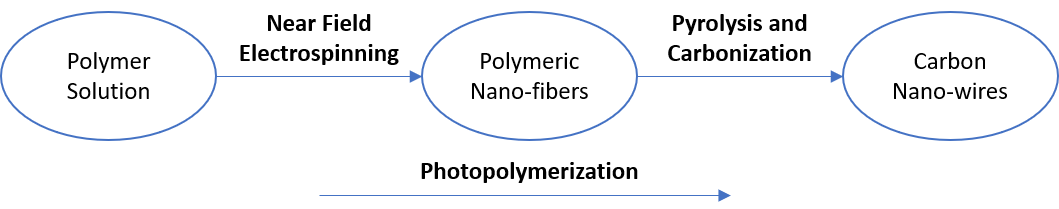
\includegraphics[width=0.95\textwidth]{./Figures/FabricationProcess.png}
%\decoRule
%\caption[Carbon Nano-wires Fabrication Process]{Fabrication process of carbon nano-wires to achieve through the proposed dissertation.}
%\label{fig:fabricationFlowChart}
%\end{figure}

%\begin{equation}
%\left(\tau _t^e-\frac{\tau _n^e \text{dr}}{\text{dz}}\right) 2 \pi  r+\frac{d \left(\pi  r^2
%   \left(\tau _{\text{zz}}-p\right)\right)}{\text{dz}}+\frac{\gamma  \text{dr} 2 \pi  r}{r
%   \text{dz}}+\rho  g \pi  r^2=\frac{d \left(\rho  \pi  r^2 v^2\right)}{\text{dz}}
%\label{eq:linearMomentum}
%\end{equation}